% Please make sure you insert your
% data according to the instructions in PoSauthmanual.pdf
\documentclass{PoS}

\usepackage{amsmath}
\usepackage{siunitx}
\usepackage{multirow}
\usepackage{lineno}
\usepackage{graphicx}
%\usepackage[utf8]{inputenc}
%\usepackage[no-math]{fontspec}
%\setmainfont{STIX}
%\usepackage{stix}

\usepackage{skeleton-defs}
\usepackage{latex/atlasunit}
\usepackage{latex/atlasparticle}
\usepackage{latex/atlasjournal}
\usepackage{latex/atlasmisc}
\usepackage{latex/atlasphysics}
%\usepackage{latex/atlaspackage}

\title{Messurement of inclusive cross section and observation of electroweak production of two jets in association with a $Z$-boson pair
in $pp$ collisions at $\sqrt{s} = 13$~\TeV~with the ATLAS detector
}

\ShortTitle{SM ZZjj analysis}

\author{\speaker{Heling Zhu, on behalf of the ATLAS Collaboration}\\
        University of Science and Technology of China, Brookhaven National Lab\\
        E-mail: \email{heling.zhu@cern.ch}}

\abstract{
    The observation of electroweak production of two jets in association with a $Z$-boson pair
    using 139 \ifb~of $pp$ collision data at $\sqrt{s} =$ 13 \TeV~collected by the ATLAS detector at the LHC is presented.
    Two different final states originating from the decays of the $Z$ boson pair,
    one containing four charged leptons, and the other two charged leptons and two neutrinos, are considered.
    A significant deviation from the background-only hypothesis is observed,
    which corresponds to a statistical significance of 5.5 $\sigma$.
    The observed excess is compatible with the electroweak production of two jets in association with a $Z$-boson pair.
    In addition, cross-sections for inclusive production of $ZZ$ plus two jets,
    as well as the observed signal strength of the EW production, are reported.
}

\FullConference{Corfu Summer Institute 2019 "School and Workshops on Elementary Particle Physics and Gravity" (CORFU2019)\\
		31 August - 25 September 2019\\
		Corfù, Greece}

\begin{document}
\linenumbers

%-------------------------------------------------------------------------------
\section{Introduction}
\label{sec:intro}
After the discovery of the Higgs boson~\cite{HIGG-2012-27,CMS-HIG-12-028}, the scrutiny of the electroweak symmetry breaking (EWSB) becomes a main focus at the LHC. In addition to direct measurements of Higgs boson properties, the study of massive vector-boson scattering (VBS) offers another key avenue to probe the EWSB~\cite{Lee:1977yc,Chanowitz:1985hj,Szleper:2014xxa}. In the Standard Model (SM), the Higgs boson acts rigorously to prevent longitudinal VBS amplitudes from violating unitarity at the \TeV~scale~\cite{Lee:1977yc}; therefore, the study of high-energy behaviours of VBS is crucial to understand the nature of the EWSB. Many new physics scenarios, such as Supersymmetry and Little Higgs models~\cite{ArkaniHamed:2002qy}, offer alternative EWSB mechanisms, which can manifest themselves as appearance of heavy particles or modifications of Higgs couplings in the accessible energy regime.
These new phenomena could manifest themselves in rises of amplitudes or resonant structures in the TeV range and thereby alter the way of delicate cancellations at high energies.

While no VBS processes were established prior to the LHC era, the LHC provides an unprecedented opportunity to study them, owing to its high collision energies and luminosities. At the LHC, VBS is typically produced as two vector bosons radiated from initial-state quarks and then scattering into another pair of vector bosons. The detector signature of VBS contains decay products of the pair of outgoing bosons and a pair of hadronic jets, hereafter denoted as $VVjj$. The most promising channel to measure VBS is therefore the electroweak (EW) production of $VVjj$ (EW $VVjj$), which has no quantum chromodynamics (QCD) vertices at leading order (LO).
The QCD production of $VVjj$ contains two QCD vertices at the lowest order (denoted as QCD $VVjj$ processes) and constitutes an irreducible background to the searches for EW $VVjj$ production. The characteristics of EW $VVjj$ production include a large separation in rapidity between the two jets (\dyjj) as well as a significant invariant mass of the jet pair (\mjj), which are often utilized to improve the signal-to-background ratio. 

Among all the EW $VVjj$ processes with massive bosons, the EW $W^{\pm}W^{\pm}jj$ and $WZjj$ processes have been observed~\cite{Aaboud:2019nmv,Aaboud:2018ddq,Sirunyan:2017ret} using LHC Run 2 data, and no obvious deviations from the SM predictions were found. The EW $ZZjj$ production was searched for by the CMS collaboration using 36.1 \ifb~of 13 \TeV~$pp$ collision data, but no evidence was found~\cite{Sirunyan:2017fvv}. This type of rare processes has a fiducial cross-section of the order of $O(0.1)$ fb in the final states where both $Z$ bosons decay leptonically.
Despite the small rate, EW $ZZjj$ production offers a clean and competitive channel to study EWSB physics. Observation of EW $ZZjj$ production is another milestone for the physics program at the LHC. Figure~\ref{fig:diagram} depicts the typical diagrams for both the EW and QCD $ZZjj$ processes. 

This talk reports on the observation of EW $ZZjj$ (including contribution from $\gamma^*$) production by the ATLAS experiment, using the complete set of 13 \TeV~$pp$ collision data taken in LHC Run 2. The search is performed in two final states where both $Z$ bosons decay leptonically: four charged leptons with two jets (\lllljj), and two charged leptons, two neutrinos and two jets (\llvvjj).
Event selections are optimized to suppress reducible backgrounds, and fiducial cross-sections for the inclusive production of the EW and QCD processes are reported separately in individual channels.
The $ZZjj$ production involving intermediate $\tau$-leptons from $Z$ decays is considered as signal but has a negligible contribution to the selected event sample. Reducible backgrounds give minor contributions in the \lllljj channel.
In the \llvvjj channel, large missing transverse momentum (\met) is required to suppress the background from \Zjet events; other major backgrounds are the production of $WWjj$, $WZjj$ and \ttbar.
To enhance the separation between the EW signal and the main backgrounds, multivariate discriminants (MDs) are trained from event kinematic information using simulated samples.
The MD distributions are fitted simultaneously in the two channels to evaluate the contribution from EW processes.


\begin{figure}[!htbp]
\begin{center}
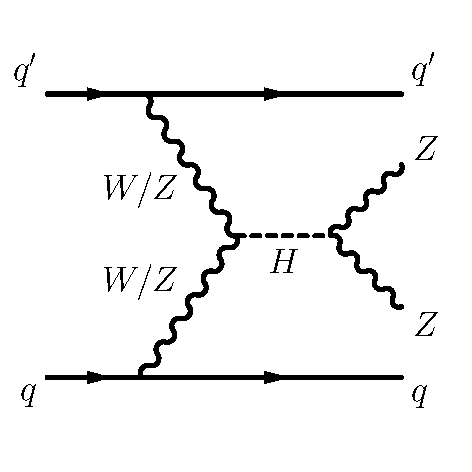
\includegraphics[width=0.22\textwidth]{figures/diagram/diagram-EWZZjj-Schn-Higgs.pdf}
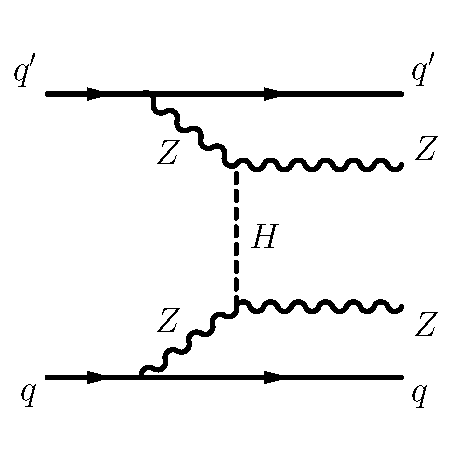
\includegraphics[width=0.22\textwidth]{figures/diagram/diagram-EWZZjj-Tchn-Higgs.pdf}
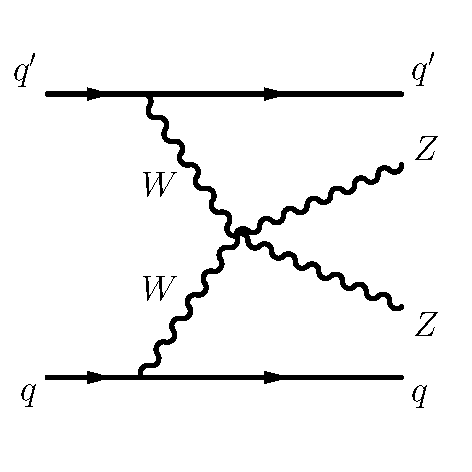
\includegraphics[width=0.22\textwidth]{figures/diagram/diagram-EWZZjj-QGC.pdf}
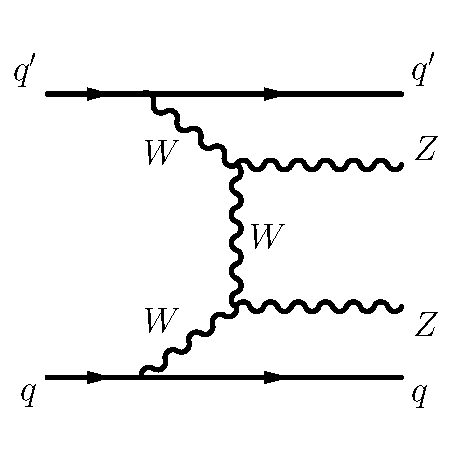
\includegraphics[width=0.22\textwidth]{figures/diagram/diagram-EWZZjj-TGC.pdf}\\
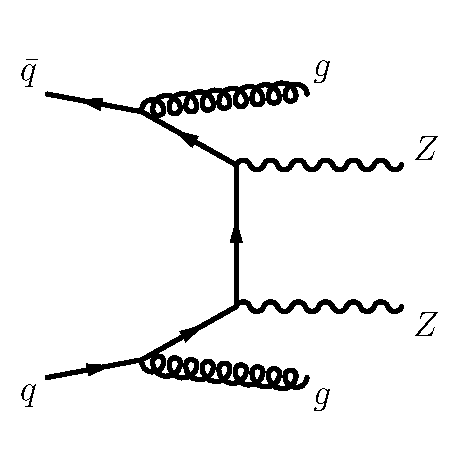
\includegraphics[width=0.22\textwidth]{figures/diagram/diagram-QCDZZjj-qq.pdf}
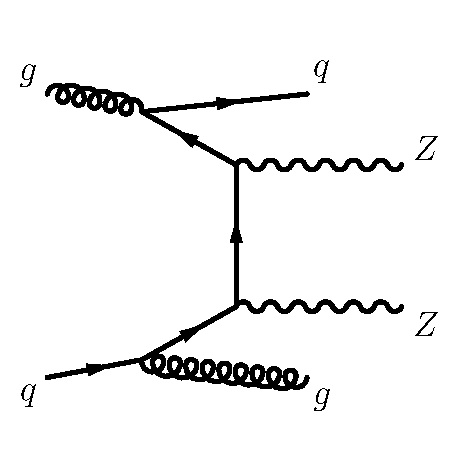
\includegraphics[width=0.22\textwidth]{figures/diagram/diagram-QCDZZjj-qg.pdf}
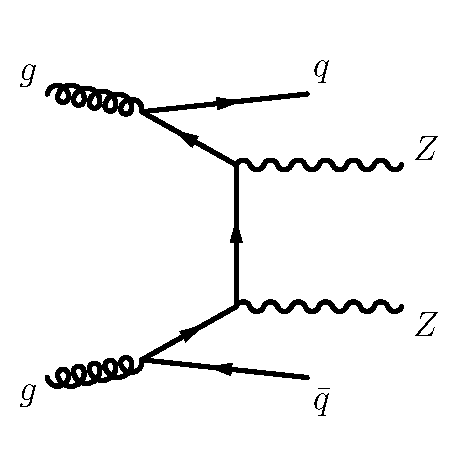
\includegraphics[width=0.22\textwidth]{figures/diagram/diagram-QCDZZjj-gg.pdf}
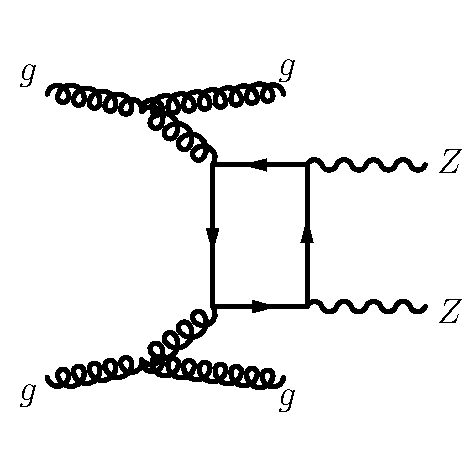
\includegraphics[width=0.22\textwidth]{figures/diagram/diagram-QCDZZjj-box.pdf}\\
\end{center}
\caption{Typical diagrams for the production of $ZZjj$, including the relevant EW VBS diagrams (first row) and QCD diagrams (second row).}
\label{fig:diagram}
\end{figure}


%-------------------------------------------------------------------------------
\section{ATLAS detector}
\label{sec:detector}
\newcommand{\AtlasCoordFootnote}{%
ATLAS uses a right-handed coordinate system with its origin at the nominal interaction point (IP)
in the centre of the detector and the \(z\)-axis along the beam pipe.
The \(x\)-axis points from the IP to the centre of the LHC ring,
and the \(y\)-axis points upwards.
Cylindrical coordinates \((r,\phi)\) are used in the transverse plane, 
\(\phi\) being the azimuthal angle around the \(z\)-axis.
The pseudorapidity is defined in terms of the polar angle \(\theta\) as \(\eta = -\ln \tan(\theta/2)\).
Angular distance is measured in units of \(\Delta R \equiv \sqrt{(\Delta\eta)^{2} + (\Delta\phi)^{2}}\).}

The ATLAS experiment~\cite{PERF-2007-01,ATLAS-TDR-2010-19,Abbott:2018ikt} at the LHC is a multi-purpose particle detector
with a forward-backward symmetric cylindrical geometry and a near \(4\pi\) coverage in 
solid angle.\footnote{\AtlasCoordFootnote}
It consists of an inner tracking detector (ID) surrounded by a thin superconducting solenoid
providing a \SI{2}{\tesla} axial magnetic field, electromagnetic and hadron calorimeters, and a muon spectrometer.
The inner tracking detector covers the pseudorapidity range \(|\eta| < 2.5\).
It consists of silicon pixel, silicon microstrip, and transition radiation tracking detectors.
Lead/liquid-argon (LAr) sampling calorimeters provide electromagnetic (EM) energy measurements
with high granularity.
A hadron (steel/scintillator-tile) calorimeter covers the central pseudorapidity range (\(|\eta| < 1.7\)).
The end-cap and forward regions are instrumented with LAr calorimeters
for both EM and hadronic energy measurements up to \(|\eta| = 4.9\).
The muon spectrometer (MS) surrounds the calorimeters and is based on
three large air-core toroidal superconducting magnets with eight coils each.
The field integral of the toroids ranges between \num{2.0} and \SI{6.0}{\tesla\metre}
across most of the detector. 
The muon spectrometer includes a system of precision tracking chambers and fast detectors for triggering.
A two-level trigger system~\cite{TRIG-2016-01} is used to select events for offline analysis. 
The first-level trigger is implemented in hardware and uses a subset of the detector information. 
This is followed by the software-based high-level trigger, that reduces the event rate to about 1 kHz.


%-------------------------------------------------------------------------------
\section{Data and simulation}
\label{sec:datamc}
The data sets for this analysis were recorded using single and multi-lepton triggers.
The transverse momentum (\pT) thresholds of these triggers vary from 8 to 26~\GeV{},
depending on the lepton flavour and data-taking periods.
The overall trigger efficiency for selected inclusive $ZZjj$ signal events in the analysis region ranges from 95 to 99\%{}.
After removing the short data-taking periods with problems affecting the lepton reconstruction,
the total integrated luminosity used in the analysis is 139 \ifb.

The EW $ZZjj$ production is modelled using \MGMCatNLO~2.6.1~\cite{Alwall:2014hca} matrix elements (ME) calculated in the LO approximation
in perturbative QCD (pQCD) and with NNPDF2.3LO~\cite{Ball:2012cx} parton distribution functions (PDF).
The QCD $ZZjj$ production is modelled using \textsc{Sherpa} 2.2.2~\cite{Gleisberg:2008ta} with the NNPDF3.0NNLO~\cite{ball2015parton} PDF,
where events with up to one (three) outgoing partons are generated at NLO (LO) in pQCD.
The production of $ZZjj$ from the gluon-gluon initial state with a four-fermion loop or with an exchange of the Higgs boson has an order of $\alpha_{S}^{4}$ in QCD,
and is not included in the \textsc{Sherpa} simulation.
This process, denoted as the $ggZZjj$ process, is modelled using \textsc{Sherpa} 2.2.2 with the NNPDF3.0NNLO PDF in the \lllljj channel,
and using \textsc{gg2VV}~\cite{Kauer:2013qba} with the CT10NNLO PDF~\cite{Gao:2013xoa} in the \llvvjj channel.
Due to the limited accuracy of ME calculation, the second (both) jets in $ggZZjj$ events are produced in parton showering in the \lllljj (\llvvjj) channel.
The leptonic decays of $Z$ bosons are included in the simulation.
Interference between EW and QCD $ZZjj$ is modelled with \MGMCatNLO~2.6.1 calculated at LO. 

The production of QCD $WWjj$ as well as EW and QCD $WZjj$ with the subsequent leptonic decays of vector bosons are modelled with \textsc{Sherpa} 2.2.2 with NNPDF3.0NNLO PDF.
Diboson processes with the subsequent semileptonic decays ($WW \rightarrow lvqq$ and $WZ \rightarrow qqll$)
are modelled using \textsc{Powheg-Box}~v2~\cite{Frixione:2007nw} with the CT10 PDF~\cite{Lai:2010vv}.
Triboson production is modelled using \textsc{Sherpa} 2.2.2 with NNPDF3.0NNLO PDF.
For top-quark pair production, the \textsc{Powheg-Box}~v2 event generator with the CT10 PDF is used.
The production of single top-quark in $t$-channel, $s$-channel and $Wt$-channel were simulated using the \textsc{Powheg-Box}~v1 event generator~\cite{Alioli:2009je,Frederix:2012dh,Re:2010bp}.
The production of \ttbar~in association with vector bosons ($ttV$) is modelled with \MGMCatNLO~2.3.3 for $ttW$ and $ttZ$ with the $Z$ to $\nu\nu/qq$ decays,
with \MGMCatNLO~2.2.2 for $ttWW$, and with \textsc{Sherpa} 2.2.1 for $ttZ$ with the $Z$ to dilepton decays, respectively.
The \Zjet processes are modelled using \textsc{Sherpa} 2.2.1 with NNPDF3.0NNLO PDF, where the ME is calculated for up to two partons with next-to-leading-order (NLO) accuracy in pQCD and up to four partons with LO accuracy.

The parton showering is modelled with \textsc{Pythia}~8.186~\cite{Sjostrand:2007gs} using NNPDF2.3~\cite{Ball:2012cx} PDF and the A14 set of tuned parameters~\cite{ATL-PHYS-PUB-2014-021}
for all the samples except for those from \textsc{Sherpa}, where parton showering is simulated within the \textsc{Sherpa} programme.

All simulated events were processed with a detailed detector simulation~\cite{SOFT-2010-01} based on \textsc{Geant4}~\cite{Agostinelli:2002hh}.
Furthermore, simulated inelastic $pp$ collisions were overlaid to model additional $pp$ collisions in the same and neighbouring bunch crossings~(pileup).
Simulated events were reweighted to match the pileup conditions in the data. All simulated events were processed using the same reconstruction algorithms as used in data.
Furthermore, the lepton and jet momentum scale and resolution, and the lepton reconstruction, identification, isolation and trigger efficiencies in the simulation were corrected to match those measured in data.




%-------------------------------------------------------------------------------
\section{Event selection}
\label{sec:sel}
The data sets for this analysis were recorded using single and multi-lepton triggers.
The transverse momentum (\pT) thresholds of these triggers vary from 8 to 26~\GeV{},
depending on the lepton flavour and data-taking periods.
The overall trigger efficiency for selected inclusive $ZZjj$ signal events in the analysis region ranges from 95 to 99\%{}.
After removing the short data-taking periods with problems affecting the lepton reconstruction,
the total integrated luminosity used in the analysis is 139 \ifb.

The selection of the \lllljj and \llvvjj events relies on multiple physics objects, including electrons, muons, jets, and \met.
Events are first required to have a collision vertex associated with at least two tracks each with $\pt>0.4$ \GeV.
The vertex with the highest scalar sum of \pt{} of the associated tracks is referred to as the primary vertex.

Muons are identified by tracks reconstructed in the MS and are matched to tracks reconstructed in the ID. In the region $2.5<|\eta|<2.7$, muons can also be identified by an MS track alone (denoted as stand-alone muons).
The identified muons described above are required to have \pT{} $>$ 7~\GeV{}.
In the MS gap region ($|\eta|<0.1$) muons are identified by an ID track with \pT{} $>$ 15~\GeV{}
associated with a compatible calorimeter energy deposit (denoted calorimeter-tagged muons).
Muons are required to have $|\eta| <$ 2.7 (2.5) and satisfy `loose' (`medium') identification criterion~\cite{PERF-2015-10} in the \lllljj (\llvvjj) channel. 

Electrons are reconstructed from energy deposits in the electromagnetic calorimeter matched to a track in the ID.
The electron identification imposes requirements on the number of hits in the ID and on a likelihood discriminant,
built from variables related to EM calorimeter shower shapes, track-cluster matching, track quality, and transition radiation.
Electrons must satisfy the `loose' (`medium') identification criterion~\cite{Aaboud:2019ynx} in the \lllljj (\llvvjj) channel, and have \pT{} $>$ 7~\GeV{} and $|\eta| < 2.47$.

All electrons and muons are required to be isolated by requiring low activity in regions of the ID and calorimeters that surround them,
and the `FixedCutLoose' and `loose' isolation criteria~\cite{PERF-2015-10,Aaboud:2019ynx} are imposed in the \lllljj and \llvvjj channels, respectively. Furthermore, leptons are required to have associated tracks satisfying $|d_0/\sigma_{d_0}|<5~(3)$ and $|z_0\times\sin\theta|<0.5$ mm for electrons~(muons), where $d_0$ is the transverse impact parameter relative to the beam line, $\sigma_{d_0}$ is its uncertainty, and $z_0$ is the longitudinal impact parameter relative to the primary vertex.

Jets are clustered using the anti-$k_t$ algorithm~\cite{antikt_algorithm,Fastjet} with radius parameter $R = 0.4$. The jet energy scale is calibrated using simulation and further corrected with in-situ methods~\cite{Aaboud:2017jcu}. 
A jet-vertex tagger~\cite{PERF-2014-03} is applied to jets with $\pT<60$~\GeV\ and $|\eta|<2.4$ to preferentially select jets from the hard interaction. In addition, jets containing $b$-hadrons ($b$-jets) are identified using a multivariate algorithm ($b$-tagging)~\cite{bjets}. The chosen $b$-tagging algorithm has an efficiency of 85\%{} for $b$-jets and a rejection factor of 33 against light-flavour jets.

An overlap-removal procedure detailed in Ref.~\cite{Aad:2016eki} is applied to the selected leptons and jets in the \llvvjj channel,
to avoid ambiguities in the event selection and in the energy measurement of the physics objects.
A similar approach is adopted in the \lllljj channel, except that leptons are given a higher priority to be kept when overlapping with jets, to enhance the selection efficiency.
The $\vec{E}_{\mathrm{T}}^{\mathrm{miss}}$ vector is computed as the negative of the vector sum of transverse momenta of all the leptons and jets, as well as the tracks originating from the primary vertex but not associated with any of the leptons or jets (``soft-term'')~\cite{ATL-PHYS-PUB-2015-027}. The soft-term is computed such that it minimises the impact of pile-up in the \met{} reconstruction. The statistical significance of \met~is built using resolution information of physics objects used in the \met~reconstruction~\cite{ATLAS-CONF-2018-038}.

In the \lllljj channel, quadruplets of leptons are formed by selecting two opposite-sign, same-flavour (OSSF) lepton pairs ($\ell^+\ell^-$), where the leptons are required to be separated from each other by $\Delta R >0.2$.
At most one muon is allowed to be a stand-alone or calorimeter-tagged muon, and the three leading leptons must have \pt{} $>$ 20, 20 and 10~\GeV{}, respectively.
If multiple quadruplets are found, the one that minimises the sum of the differences between the dilepton masses and the nominal $Z$ boson mass,
$|m_{\ell^+\ell^-} - m_Z| + |m_{\ell^{'+}\ell^{'-}} - m_Z|$, is selected.
The dilepton masses are required to be within 66--116~\GeV{}.
In the \lllljj channel with four electrons ($4e$) or four muons ($4\mu$), all the $\ell^+\ell^-$ pairs are required to have $m_{\ell^+\ell^-} > 10$~\GeV{},
to reject events with low mass resonances. 

In the \llvvjj channel candidate events  are required to have one OSSF lepton pair with $m_{\ell^+\ell^-}$ in the range from 80 to 100~\GeV{},
and the leading (sub-leading) lepton must have \pt{} $>$ 30 (20)~\GeV{}.
Events with $b$-tagged jets or additional leptons (\pt{} $>$ 7~\GeV{} and satisfying `loose' requirement) are rejected, to reduce the background contributions from \ttbar~and $WZ$ events.
Events should satisfy the requirement of \met-significance greater than 12 to suppress the background from \Zjet processes.

In both channels, the two most energetic jets satisfying $y_{j_1} \times y_{j_2} < 0$ are selected.
In the \lllljj channel the jets are required to have \pT $>$ 30~(40)~\GeV{} in the $|\eta| < 2.4 (2.4 < |\eta| < 4.5)$ region,
while in the \llvvjj channel the selected jets are required to have \pT $>$ 60 (40)~\GeV{} for the leading (sub-leading) one.
Finally, to further suppress background contributions, \mjj is required to be greater than 300 (400)~\GeV{} in the \lllljj (\llvvjj) channel, and \dyjj is required to be greater than 2.
The harsher jet requirement in the \llvvjj channel is optimised to suppress the more significant contamination from reducible backgrounds. 

The analysis signal regions (SRs), defined with the above selection requirements, are summarized in Table~\ref{tab:selection_reco}.

\begin{table}[!htbp]
\begin{center}
\scalebox{0.75} {
\begin{tabular}{c c c}
\hline
\hline \noalign{\smallskip}
        & \lllljj                                                                            & \llvvjj                                                            \\
\noalign{\smallskip}\hline\noalign{\smallskip}
\multirow{2}{*}{Electrons} & \multicolumn{2}{c}{$\pT >$ 7~\GeV{}, $|\eta| <$ 2.47}                                   \\
                     & \multicolumn{2}{c}{$|d_0/\sigma_{d_0}|<5$ and $|z_0\times\sin\theta|<0.5$ mm}                                                              \\
\noalign{\smallskip}\hline\noalign{\smallskip}
\multirow{2}{*}{Muons}         & $\pT >$ 7~\GeV{}, $|\eta| <$ 2.7                                                 & $\pT >$ 7~\GeV{}, $|\eta| <$ 2.5             \\
                     & \multicolumn{2}{c}{$|d_0/\sigma_{d_0}|<3$ and $|z_0\times\sin\theta|<0.5$ mm}                                                              \\
\noalign{\smallskip}\hline\noalign{\smallskip}
Jets      & $\pT >$ 30 (40)~\GeV{} for $|\eta| <$ 2.4 ($2.4<|\eta|<4.5$)                   & $\pT >$ 60 (40)~\GeV{} for the leading (sub-leading) jet               \\ 
\noalign{\smallskip}\hline\noalign{\smallskip}
\multirow{5}{*}{$ZZ$ selection}  & $\pT >$ 20, 20, 10~\GeV{} for the leading, sub-leading and third leptons     & $\pT >$ 30 (20)~\GeV{} for the leading (sub-leading) lepton  \\
                     & Two OSSF lepton pairs with smallest $|m_{\ell^+\ell^-} - m_Z| + |m_{\ell^{'+}\ell^{'-}} - m_Z|$   & One OSSF lepton pair and no third leptons    \\
                     & $m_{\ell^+\ell^-} >$ 10~\GeV{} for lepton pairs                                      & 80 $< m_{\ell^+\ell^-} <$ 100~\GeV{}                             \\
                     & $\Delta R(\ell,\ell') >$ 0.2                                                         & No b-tagged jets                                             \\
                     & 66 $< m_{\ell^+\ell^-} <$ 116~\GeV{}                                                  & \met significance $>$ 12                                     \\
\noalign{\smallskip}\hline\noalign{\smallskip}
\multirow{2}{*}{Dijet selection}  & \multicolumn{2}{c}{Two most energetic jets with $y_{j_1} \times y_{j_2} < 0$}                                                        \\
                     & \mjj $>$ 300~\GeV{} and \dyjj $>$ 2                                              & \mjj $>$ 400~\GeV{} and \dyjj $>$ 2                          \\
\noalign{\smallskip}\hline
\hline
\end{tabular}}
\end{center}
\caption{Summary of selection of physics objects and candidate events at detector level in the \lllljj and \llvvjj signal regions.}
\label{tab:selection_reco}
\end{table}


The fiducial volumes for the cross-section measurements are defined closely following the detector-level selections,
using `particle-level' physics objects, which are reconstructed in simulation from stable final-state particles, prior to their interactions with the detector.
For electrons and muons, QED final-state radiation is for the most part recovered by adding to the lepton four-momentum the four-momenta of surrounding photons
not originating from hadrons within an angular distance $\Delta R < 0.1$.
Particle-level jets are built with the anti-$k_t$ algorithm with radius parameter $R = 0.4$,
using all final-state particles (excluding muons and neutrinos) as input.
Particle-level \met is defined as the vector sum of all the transverse momenta of neutrinos not originating from hadrons.
In the \lllljj channel, the dilepton mass requirement is relaxed (with respect to the detector-level selection) to be within 60 to 120~\GeV{}
to reduce the migration effect and keep compatibility with the previous CMS publication~\cite{Sirunyan:2017fvv}.
In the \llvvjj channel, both electrons and muons are selected in the $|\eta| <$ 2.5 region to simplify the lepton selections.
In addition, no requirement is applied on \met significance due to the complexity of defining this variable at `particle-level',
however, particle-level \met is required to be greater than 130~\GeV{}.
All the other kinematic selection requirements have the same definition as the detector-level ones.



%-------------------------------------------------------------------------------
\section{Background estimation}
\label{sec:bkg}
The QCD $ZZjj$ production is an irreducible background in the search for EW $ZZjj$ production.
This process is estimated from simulation via a data-driven correction for its normalization in the \lllljj channel, and estimated purely from simulation in the \llvvjj channel.
For the $gg$-initial process in $ZZjj$ channel, an additional $K$-factor of 1.7~\cite{PhysRevD.92.094028} is applied to account for the NLO QCD correction.
In the \lllljj channel, the normalization of the QCD $ZZjj$ processes is constrained by a dedicated control region (CR) defined in data by reverting either the \mjj or \dyjj requirements,
and is then included as a floating parameter in the statistical fit to properly treat the uncertainty correlations between SR and CR.
This CR cannot be defined in the \llvvjj channel, due to large contributions from reducible background.

In the \lllljj channel, background contributions from \Zjet, top-quark and $WZ$ processes are estimated from data.
These events may contain two or three isolated leptons from $Z$ or $W$ decays, together with heavy-flavour jets or misidentified components of jets yielding reconstructed leptons, i.e. `fake-leptons'.
These `fake-lepton' backgrounds are estimated using a method similar to that described in Ref.~\cite{Aaboud:2017rwm},
where the lepton misidentification is measured in data regions with enhanced contributions from \Zjet and top-quark processes.
Small background contributions from triboson and $ttV$ production are estimated from simulation.
Backgrounds from all these non-$ZZ$ processes collectively yield an contribution of about 3\% to the selected data sample. These minor backgrounds are hereafter referred to as ``Others'' in the \lllljj channel.

In the \llvvjj channel, the QCD $ZZjj$ processes constitute 26\% of the selected sample,
and the remaining major backgrounds originate from $WZjj$ (29\%), $WWjj$ and \ttbar~production (27\%).
The shape of $WZjj$ background is estimated from MC simulation, 
while its normalization is then fixed using a data CR defined by requiring three selected leptons and a looser event selection, following the methodology explained in Ref.~\cite{Aaboud:2017bja}.
The simulation is found to overestimate the $WZjj$ contribution by 15\% in this CR in data,
and therefore, the $WZjj$ yield in the SR is scaled by 0.85.
The $WZjj$ estimate is found to have a relative uncertainty of 5\%, due to the data statistical uncertainty in the CR as well as the experimental and theoretical uncertainties.
The $WZjj$ distribution of the MD is evaluated from simulation with the EW $WZjj$ normalisation scaled by 1.77, corresponding to the difference between data and simulation observed in a previous analysis, in a similar phase space~\cite{Aaboud:2018ddq},
where the overall normalization factor is found to be consistent with the one derived in this note.
The $WZjj$ shape uncertainty originates from experimental and theoretical uncertainties as well as from the uncertainty in the quoted EW $WZjj$ cross-section measurement.
The \nonresll~background, including the $WWjj$ and \ttbar~processes, contain genuine \met~and a lepton pair not originating from a $Z$ decay.
This background is estimated using a CR selected in data by requiring the same selection as in the SR with the exception that an $e\mu$ pair is required, following the methodology explained in Ref.~\cite{Aaboud:2017bja}.
The \nonresll~estimate has a relative uncertainty of 20\%, dominated by the data statistical uncertainty in the CR.
The MD distribution for the \nonresll~process is estimated from simulation,
with an uncertainty assigned to account for the difference between shapes in data and simulation.
The \Zjet background is largely suppressed, and the yield is evaluated by extrapolating the low \met-significance region distribution in data to the high \met-significance region using an exponential function,
while the MD distribution in the SR is modeled by simulation.
A conservative uncertainty is assigned to account for variations in the fitting functions as well as differences between estimated and simulated yields and distributions.
In addition, triboson and $ttV$ backgrounds are modelled with simulation. Similar to the \lllljj channel, these minor backgrounds are denoted as ``Others''.

The observed and expected yields are listed in Table~\ref{tab:yield_prefit},
where in total 127 (82) data events are selected in the \lllljj (\llvvjj) channel.
No significant deviation from the SM prediction is observed.

\begin{table}[!htbp]
\sisetup{
table-number-alignment = center,
table-align-uncertainty=true
}
\begin{center}

% \begin{tabular}{c|c|c}
% \hline
% Process                 & \lllljj          & \llvvjj           \\
% \hline
% EW $ZZjj$               &  $20.6 \pm  2.5$ & $12.3 \pm 0.7$  \\
% QCD $ZZjj$              &  $77.4 \pm 25.0$ & $17.2 \pm 3.5$  \\
% QCD $ggZZjj$            &  $13.1 \pm  4.4$ & $ 3.5 \pm 1.1$  \\
% Non-resonant-$\ell\ell$ &  -               & $21.4 \pm 4.8$  \\
% $WZ$                    &  -               & $22.8 \pm 1.1$  \\
% Others                  &  $ 3.2 \pm  2.1$ & $ 1.2 \pm 0.9$  \\
% \hline
% Total                   & $114.3 \pm 25.6$ & $78.4 \pm 6.2$  \\
% \hline
% Data                    &  127             & 82              \\
% \hline
% \end{tabular}


\begin{tabular}{
c
S[table-format = 3.1]@{$\,\pm\,$}
S[table-format = 2.1]
S[table-format = 2.2]@{$\,\pm\,$}
S[table-format = 1.2]
}
%\hline
%Process                 & \multicolumn{2}{c}{\lllljj}    & \multicolumn{2}{c}{\llvvjj}           \\
%\hline
%EW $ZZjj$               &  20.6 &  2.5 & 12.3 & 0.7  \\
%QCD $ZZjj$              &  77.4 & 25.0 & 17.2 & 3.5  \\
%QCD $ggZZjj$            &  13.1 &  4.4 & 3.5 & 1.1  \\
%Non-resonant-$\ell\ell$ &  \multicolumn{2}{c}{-} & 21.4 & 4.8  \\
%$WZ$                    &  \multicolumn{2}{c}{-} & 22.8 & 1.1  \\
%Others                  &   3.2 &  2.1 & 1.2 & 0.9  \\
%\hline
%Total                   & 114.3 & 25.6 & 78.4 & 6.2  \\
%\hline
%Data                    &  \multicolumn{2}{l}{127}    & \multicolumn{2}{l}{82}  \\
%\hline
%\end{tabular}
\hline
Process                 & \multicolumn{2}{c}{\lllljj}    & \multicolumn{2}{c}{\llvvjj}           \\
\hline
EW $ZZjj$               &  20.6 &  2.5 & 12.30 & 0.65  \\
QCD $ZZjj$              &  77   & 25   & 17.2  & 3.5  \\
QCD $ggZZjj$            &  13.1 &  4.4 &  3.5  & 1.1  \\
Non-resonant-$\ell\ell$ &  \multicolumn{2}{c}{-} & 21.4 & 4.8  \\
$WZ$                    &  \multicolumn{2}{c}{-} & 22.8 & 1.1  \\
Others                  &   3.2 &  2.1 & 1.15  & 0.89  \\
\hline
Total                   & 114   & 26   & 78.4 & 6.2  \\
\hline
Data                    &  \multicolumn{2}{l}{127}    & \multicolumn{2}{l}{82}  \\
\hline
\end{tabular}


\end{center}
\caption{
Observed data and expected signal and background yields in 139~\ifb{} of data.
Minor backgrounds are summed together as `Others'.
Uncertainties on the predictions include both statistical and systematic components.
}
\label{tab:yield_prefit}
\end{table}




%-------------------------------------------------------------------------------
\section{Uncertainties}
\label{sec:unc}
This analysis performs cross-section measurements in the fiducial volumes as well as a statistical fit to MD distributions to extract the EW $ZZjj$ contributions. Therefore, experimental and theoretical uncertainties may influence the analysis in the predictions of background yields and MD shapes,
correction factors to extrapolate the QCD and EW $ZZjj$ events from detector-level to fiducial volume
(i.e. $C$-factors, calculated as the ratio of the number of $ZZjj$ events passing the detector-level event selection to the number of events selected in the fiducial volume), as well as $ZZjj$ MD shapes.
The statistical uncertainties of the simulated samples for both the signal and background processes are also taken into account.
The systematic uncertainty sources that affect $ZZjj$ production are detailed below.
%, while the uncertainties specific to background estimation will be discussed in the following section.

The major experimental uncertainties originate from the luminosity uncertainty, the momentum scale and resolution of leptons and jets,
as well as from the lepton reconstruction and selection efficiencies.
Smaller experimental uncertainties are also considered, such as those due to the trigger selection efficiency, the calculation of the \met~soft-term, the pile-up correction, and the $b$-jet identification efficiency. Overall, the total experimental uncertainty in $C$-factors~is 5--10\%, dominated by the jet and lepton components. The uncertainty in the combined 2015--2018 integrated luminosity is 1.7\%~\cite{ATLAS-CONF-2019-021}, obtained using the LUCID-2 detector \cite{LUCID2} for the primary luminosity measurements.
In addition, a conservative uncertainty is assigned on the QCD $ZZjj$ processes by comparing the MD distributions in low and high pile-up conditions, to account for a potential mismodelling of pile-up in simulation.

The theoretical uncertainties on the EW and QCD $ZZjj$ processes include the uncertainties from PDF, QCD scales, $\alpha_{S}$, and parton showering. The PDF uncertainty is estimated following the PDF4LHC~\cite{Butterworth:2015oua} procedure, where the envelope of the NNPDF internal errors and the differences between the nominal and alternative PDFs are considered as the final uncertainty.
The QCD scale uncertainty is estimated by varying independently by factors of 0.5 to 2.0 the nominal renormalisation and factorisation scales ($\mu_r$ and $\mu_f$),
which results in seven different configurations excluding the two extreme variations, ($\mu_r = 2$, $\mu_f = 0.5$) and ($\mu_r = 0.5$, $\mu_f = 2$),
where the largest deviation is chosen as the uncertainty.
The parton showering uncertainty is estimated by comparing the nominal \textsc{Pythia8} parton showering with the alternative \textsc{Herwig7}~\cite{Bellm:2015jjp, Bahr:2008pv} algorithm. The $\alpha_{S}$ uncertainty is estimated by varying the $\alpha_{S}$ value within $\pm$ 0.001. The interference effect between the EW and QCD processes is checked with \MGMCatNLO~2.6.1 at particle level, and found to be +7(+2)\% of the EW contribution in the fiducial volume in the \lllljj (\llvvjj) channel. This effect is taken as an additional uncertainty in the EW $ZZjj$ predictions. The total theoretical uncertainty in the fiducial volume yields for the EW (QCD) $ZZjj$ process is estimated to be about 10\% (30\%), where the large uncertainty in the QCD prediction is dominated by the QCD scale uncertainty.
As the shape of QCD $ZZjj$ production is critical in the determination of EW $ZZjj$ signal contributions,
an additional uncertainty affecting the MD shapes (`generator modelling uncertainty') is considered,
estimated by comparing \textsc{Sherpa} with \MGMCatNLO~2.6.1 predictions at particle level, where two partons are explicitly required in the ME calculation.



%-------------------------------------------------------------------------------
\section{Measurement of fiducial cross-sections}
\label{sec:xs}
The fiducial cross-section for the production of inclusive $ZZjj$ is measured in each channel, following the formula $\sigma = (N_{\mathrm{data}} - N_{\mathrm{bkg}}) / (L \times C)$,
where $N_{\mathrm{data}}$ and $N_{\mathrm{bkg}}$ refer to the number of events in data and expected background events, respectively, and $L$ refers to the integrated luminosity.
% and $C$ is the correction factor calculated as the ratio of the number of $ZZjj$ events passing the detector-level event selection to the number of events selected in the fiducial volume.
The $C$-factors are found to be ($69.9 \pm 0.3(\mathrm{stat}) \pm 1.2(\mathrm{theo}) \pm 2.8(\mathrm{exp})$)\% in the \lllljj channel,
and ($21.6 \pm 0.3(\mathrm{stat}) \pm 0.8(\mathrm{theo}) \pm 0.8(\mathrm{exp})$)\% in the \llvvjj channel.
The small $C$-factor in the \llvvjj channel is due to the large event migration effect,
where events passing the \met-significance requirement at detector-level could have a soft \met at particle-level.
The measured and predicted fiducial cross-sections are presented in Table~\ref{tab:xs}.
The measured cross-section has a total uncertainty of 11\% (29\%) in the \lllljj (\llvvjj) channel, and is found to be compatible with the SM prediction.
The data statistical uncertainty is dominating, while the experimental uncertainties relating to jet energy scale and resolution and the background estimations are the major systematic uncertainties in the \lllljj and \llvvjj channels, respectively.

\begin{table}[!htbp]
\begin{center}
\scalebox{0.90}{
\begin{tabular}{c | c | c}
\hline
\hline\noalign{\smallskip}  
        & Measured fiducial $\sigma$ [fb] & Predicted fiducial $\sigma$ [fb] \\
\noalign{\smallskip}\hline\noalign{\smallskip}
\lllljj & $1.27 \pm 0.12(\mathrm{stat}) \pm 0.02(\mathrm{theo}) \pm 0.07(\mathrm{exp}) \pm 0.01(\mathrm{bkg}) \pm 0.03(\mathrm{lumi})$ & $1.14 \pm 0.04(\mathrm{stat}) \pm 0.20(\mathrm{theo})$ \\
\noalign{\smallskip}\hline\noalign{\smallskip}
\llvvjj & $1.22 \pm 0.30(\mathrm{stat}) \pm 0.04(\mathrm{theo}) \pm 0.06(\mathrm{exp}) \pm 0.16(\mathrm{bkg}) \pm 0.03(\mathrm{lumi})$ & $1.07 \pm 0.01(\mathrm{stat}) \pm 0.12(\mathrm{theo})$ \\
\noalign{\smallskip}\hline
\hline
\end{tabular}}
\end{center}
\caption{
Measured and predicted fiducial cross-sections in both the \lllljj and \llvvjj channels.
Uncertainties due to different sources are presented.
}
\label{tab:xs}
\end{table}



%-------------------------------------------------------------------------------
\section{Search for electroweak $ZZjj$}
\label{sec:ewk}

Figure~\ref{fig:mjj} presents the \mjj spectra in the \lllljj and \llvvjj SRs, as well as in the \lllljj QCD $ZZjj$ CR,
where the normalization of the $ZZjj$ processes is fixed to the observed value, as explained later in this section.
This figure
%shows a good agreement between the data and the predictions,
indicates the high \mjj region as the most sensitive to EW $ZZjj$ event detection.
Figure~\ref{fig:mZZ} depicts the invariant mass of the four-lepton system ($m_{ZZ}$) in the \lllljj channel.
%The $m_{ZZ}$ is a sensitive variable to probe EWSB and that we start to be sensitive to the TeV scale.

To separate the EW $ZZjj$ processes from their backgrounds, MDs based on the Gradient Boosted Decision Tree algorithm~\cite{friedman2001} are trained with simulated events using the TMVA framework~\cite{Hocker:2007ht}. In each channel, a single MD is trained in the SR, which uses event kinematic information sensitive to the characteristics of the EW signal. In the \lllljj channel, twelve input variables are used: \mjj, \dyjj, \pt~of the leading and subleading jets (\ptleadj and \ptsubj), product of jet rapidities ($y_{j1}\times y_{j2}$), \pt~of the $Z$ boson reconstructed from the lepton pair with the mass closer to the $Z$ boson mass, rapidity of both $Z$ bosons ($y_{Z1}$ and $y_{Z2}$), \pt~and mass of the four-lepton system, \pt~of the third lepton, \pt~of the $ZZjj$ system divided by the scalar \pt~sum of $Z$ bosons and two jets ($S_{\mathrm{T}}$). Thirteen input variables are utilized in the \llvvjj channel, which are \mjj, \dyjj, $y_{j1}\times y_{j2}$, \ptsubj, \met, \met~significance, $S_{\mathrm{T}}$, pseudorapidity and azimuthal angle difference between two leptons ($\Delta\eta$, $\Delta\phi$), $\Delta R = \sqrt{(\Delta\eta)^2 + (\Delta\phi)^2}$, invariant mass of the lepton pair, and \pt~of leading and subleading leptons.
%The different set of variables in the \llvvjj channel is chosen in light of the presence of \nonresll~and $WZjj$ backgrounds, in addition to the irreducible QCD $ZZjj$ process.
The jet-related information provides the greatest sensitivity in the \lllljj channel, while both the jet-related and the dilepton-related variables are important in the \llvvjj channel. 

In the \lllljj channel the MD distributions in both the SR and the QCD $ZZjj$ CR are used in the statistical fit,
while only the MD distribution in the SR is fitted in the \llvvjj channel.
The yields of the background processes in the \llvvjj channel are determined in the CRs in data and are subsequently fixed in the statistical fit.
Figure~\ref{fig:MVA_2l2v_CR} presents the observed and predicted MD distributions in the $WZjj$ CR in the \llvvjj channel, where the predictions and the data are found to be compatible. 

To examine the compatibility of the data and the signal-plus-background hypothesis, a test statistic is defined using the profile likelihood ratio method~\cite{cowan:Asymptotic2013}.  The likelihood function is the product of all the Poisson probability density functions built in individual MD bins and across all the regions, including the \lllljj and \llvvjj SRs and the \lllljj QCD $ZZjj$ CR. In each bin the observed number of events in data is modeled by a Poisson probability density function with a mean equal to the sum of the predicted signal and background yields. The systematic uncertainties are implemented as nuisance parameters (NPs) constrained by Gaussian functions. In most cases, a common NP is used to account for each systematic uncertainty in all the bins and regions, except the the QCD scale uncertainty and generator modeling uncertainty described below. The statistical uncertainties of the simulated samples are uncorrelated among all bins, and the background uncertainties only apply to the corresponding backgrounds. The theoretical uncertainties for the $ZZjj$ production are uncorrelated between the \lllljj and \llvvjj channels, due to the different fiducial volume definitions. The QCD scale uncertainty for QCD $ZZjj$ production is treated as uncorrelated between the SR and the QCD CR in the \lllljj channel, as the two regions are selected with a large phase-space difference. Furthermore, two separate NPs are implemented to account for the generator modelling uncertainty for QCD $ZZjj$ production in the low and high MD regions.

The binning of MD distributions in the SRs is optimised to maximise the sensitivity of detecting EW $ZZjj$ events.
In the \lllljj channel, the normalisation of QCD $ZZjj$ production (\muQCD) is varied simultaneously in the fit in the SR and QCD CR.
The measured fiducial cross-section over the SM prediction for EW $ZZjj$ production (\muEW) is taken as the parameter of interest.
The effects of the uncertainties associated to normalizations and shapes of background processes in the MD distribution
are taken into account, except for theoretical uncertainties associated to the EW signal normalization,
so that the uncertainty in the fitted \muEW~directly corresponds to that in the measured fiducial cross-section.
The statistical tests are performed in both the individual \lllljj and \llvvjj channels, and in the combined channel.
The results are shown in Table~\ref{tab:fit_result}. 
To build the test statistic and to derive the expected results, observed data is used in the QCD $ZZjj$ CR in the \lllljj channel,
while in the SRs Asimov datasets are constructed from the SM predictions with \muEW $=1$ and \muQCD $=1$ in both the \lllljj and \llvvjj channels.
From the combined channel, the observed \muEW is $1.35\pm0.34$, while \muQCD is determined to be $0.96\pm0.22$.
The total systematic uncertainty in \muEW is about 0.1, while the data statistical uncertainty is 0.3.
The background-only hypothesis is rejected at 5.5 $\sigma$ (4.3 $\sigma$) from the data (expectation), leading to the observation of EW $ZZjj$ production. 
The post-fit MD distributions are shown in Figure~\ref{fig:MVA}.
The EW $ZZjj$ cross-section (combing the \lllljj and \llvvjj channels) in the fiducial volume is derived to be $0.82\pm0.21$ fb, 
which is consistent with the SM prediction of $0.61 \pm 0.03$ fb.

\begin{table}[!htbp]
\begin{center}
\begin{tabular}{c|c|c|c}
\hline
                 & $\mu_{\mathrm{EW}}$ &  $\mu^{\ell\ell\ell\ell jj}_{\mathrm{QCD}}$   &  Significance Obs. (Exp.) \\
\hline
\lllljj          & $1.54 \pm 0.42$     &  $0.95 \pm 0.22$                              &  5.48 (3.90) $\sigma$     \\
\hline
\llvvjj          & $0.73 \pm 0.65$     &  -                                            &  1.15 (1.80) $\sigma$     \\
\hline
Combined         & $1.35 \pm 0.34$     &  $0.96 \pm 0.22$                              &  5.52 (4.30) $\sigma$     \\
\hline
\end{tabular}
\end{center}
\caption{
Observed \muEW and \muQCD, as well as the observed and expected significance from the individual \lllljj and \llvvjj channels, and the combined fits.
The full set of systematic uncertainties is included.
}
\label{tab:fit_result}
\end{table}


\begin{figure}[!htbp]
\begin{center}
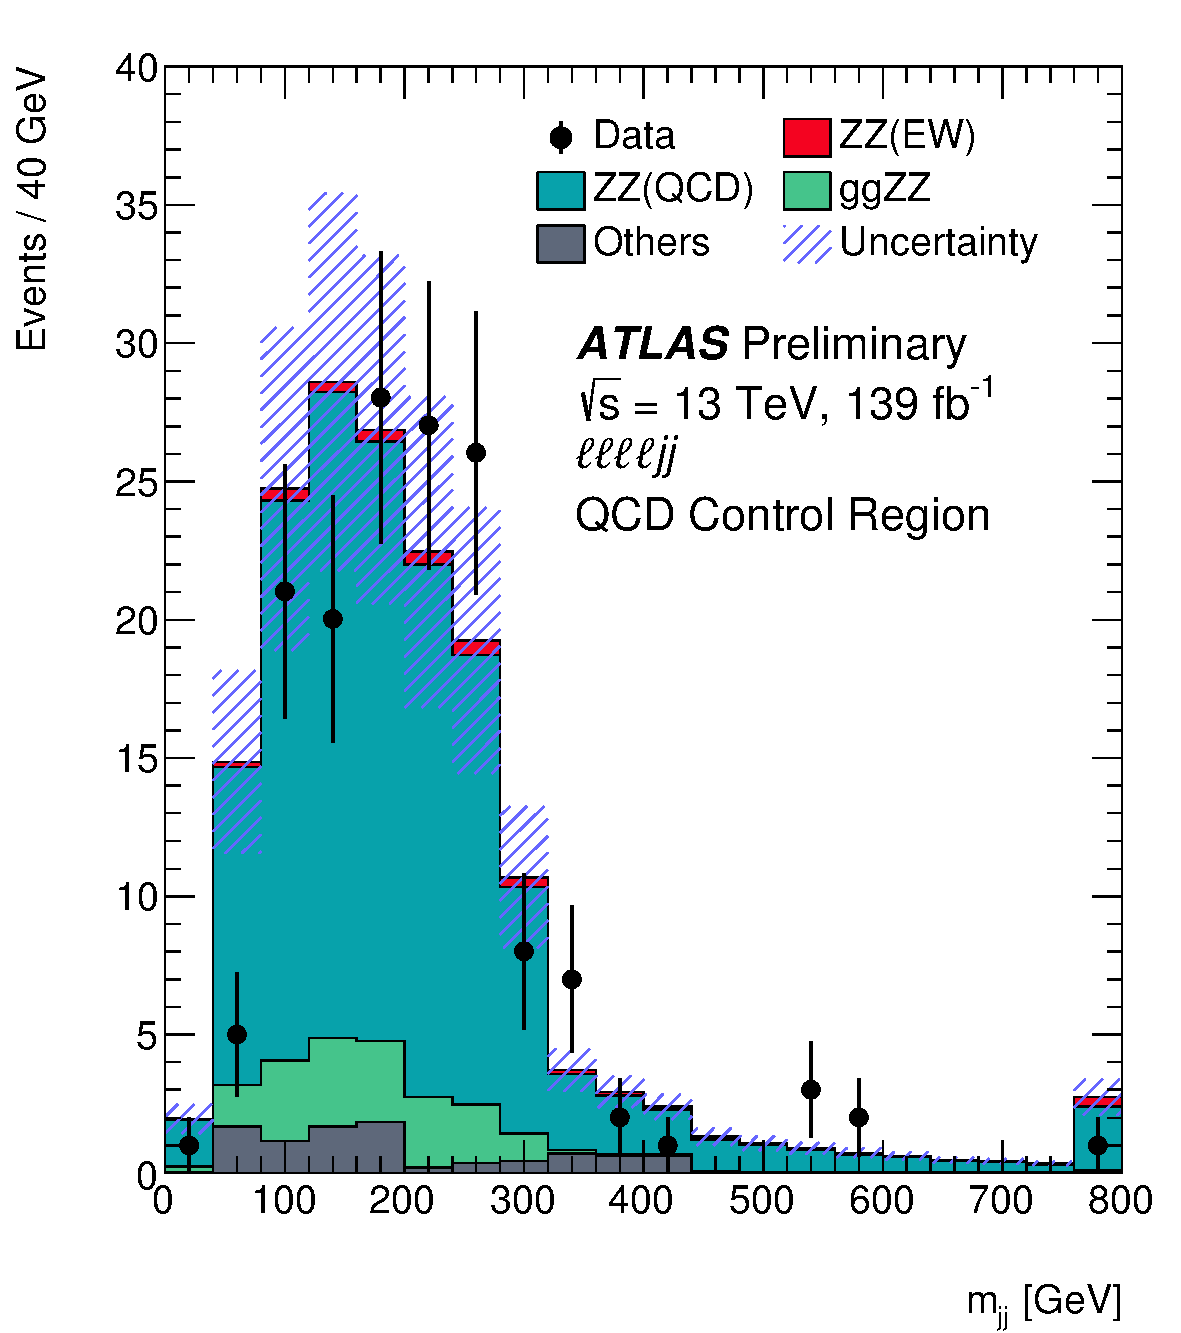
\includegraphics[width=0.325\textwidth]{figures/4l/MJJ_4l_QCD_CR_v1.pdf}
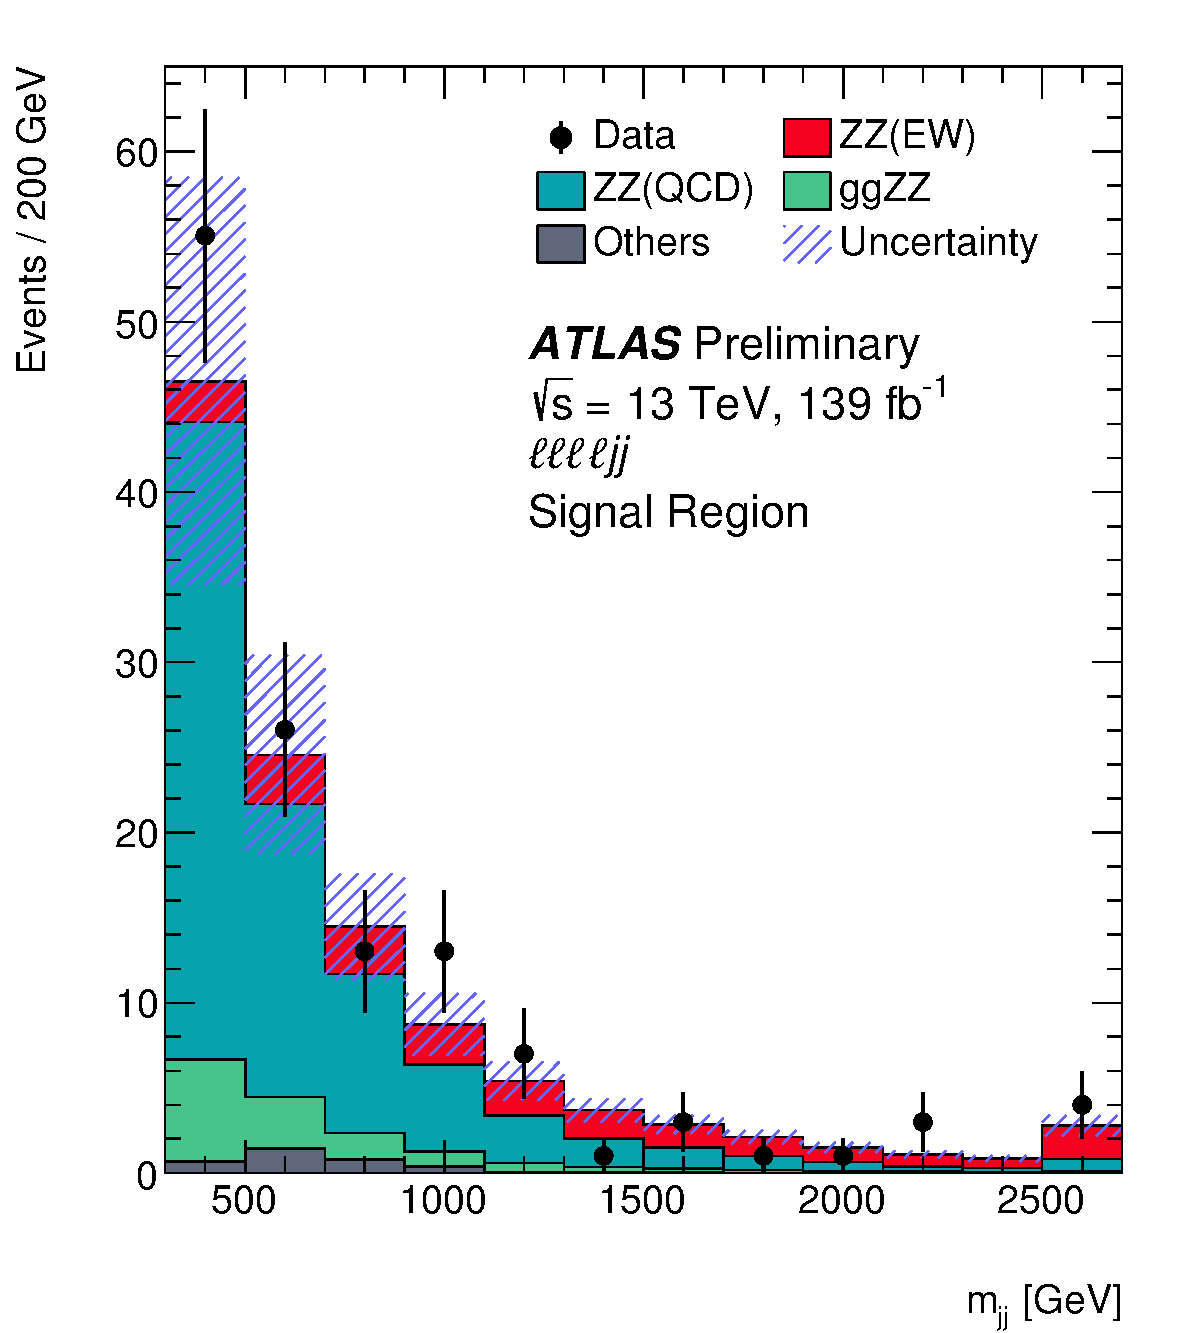
\includegraphics[width=0.325\textwidth]{figures/4l/MJJ_4l_SR_v1.pdf}
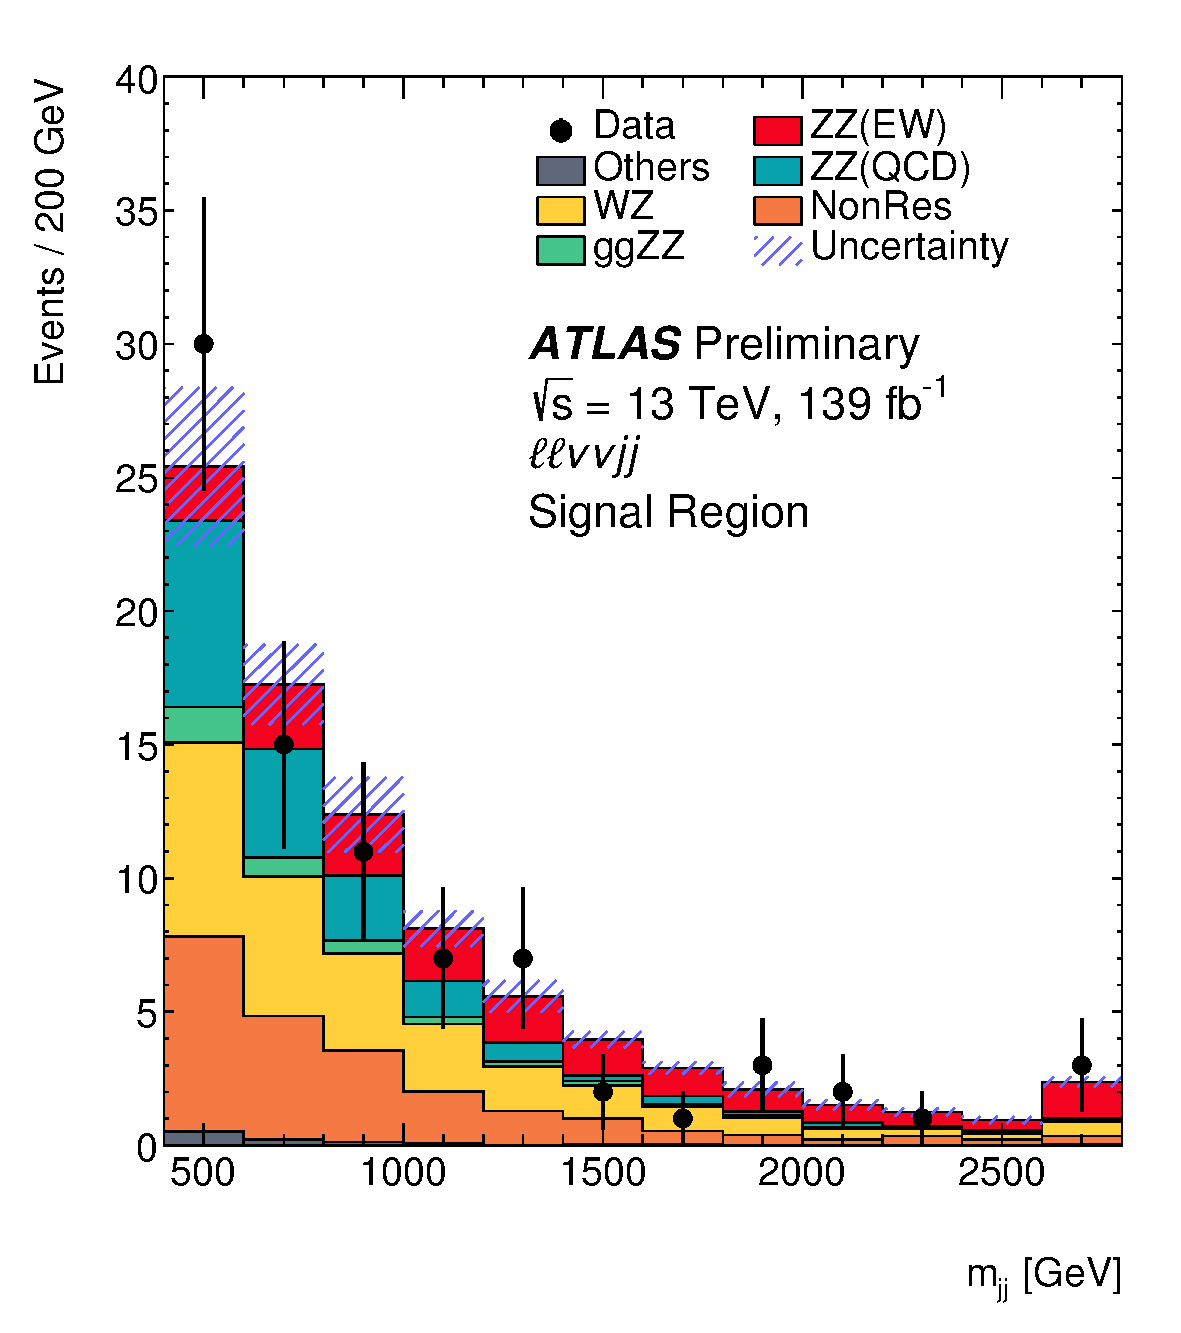
\includegraphics[width=0.325\textwidth]{figures/llvv/MJJ_2l2v_SR_v1.pdf}\\
\end{center}
\caption{Observed and expected \mjj distributions in the \lllljj QCD CR (left), 
        and in the \lllljj (middle) and \llvvjj (right) signal regions.
        The error bands include the expected experimental and theoretical uncertainties.
        The error bars on the data points show the statistical uncertainty on data.
        The contributions from the QCD and EW production of $ZZjj$ events are scaled by 0.96 and 1.35, respectively, 
        which correspond to the observed normalization factors in the statistical fit to the combined channel.
        The last bin includes the overflow events.
        }
\label{fig:mjj}
\end{figure}

\begin{figure}[!htbp]
\begin{center}
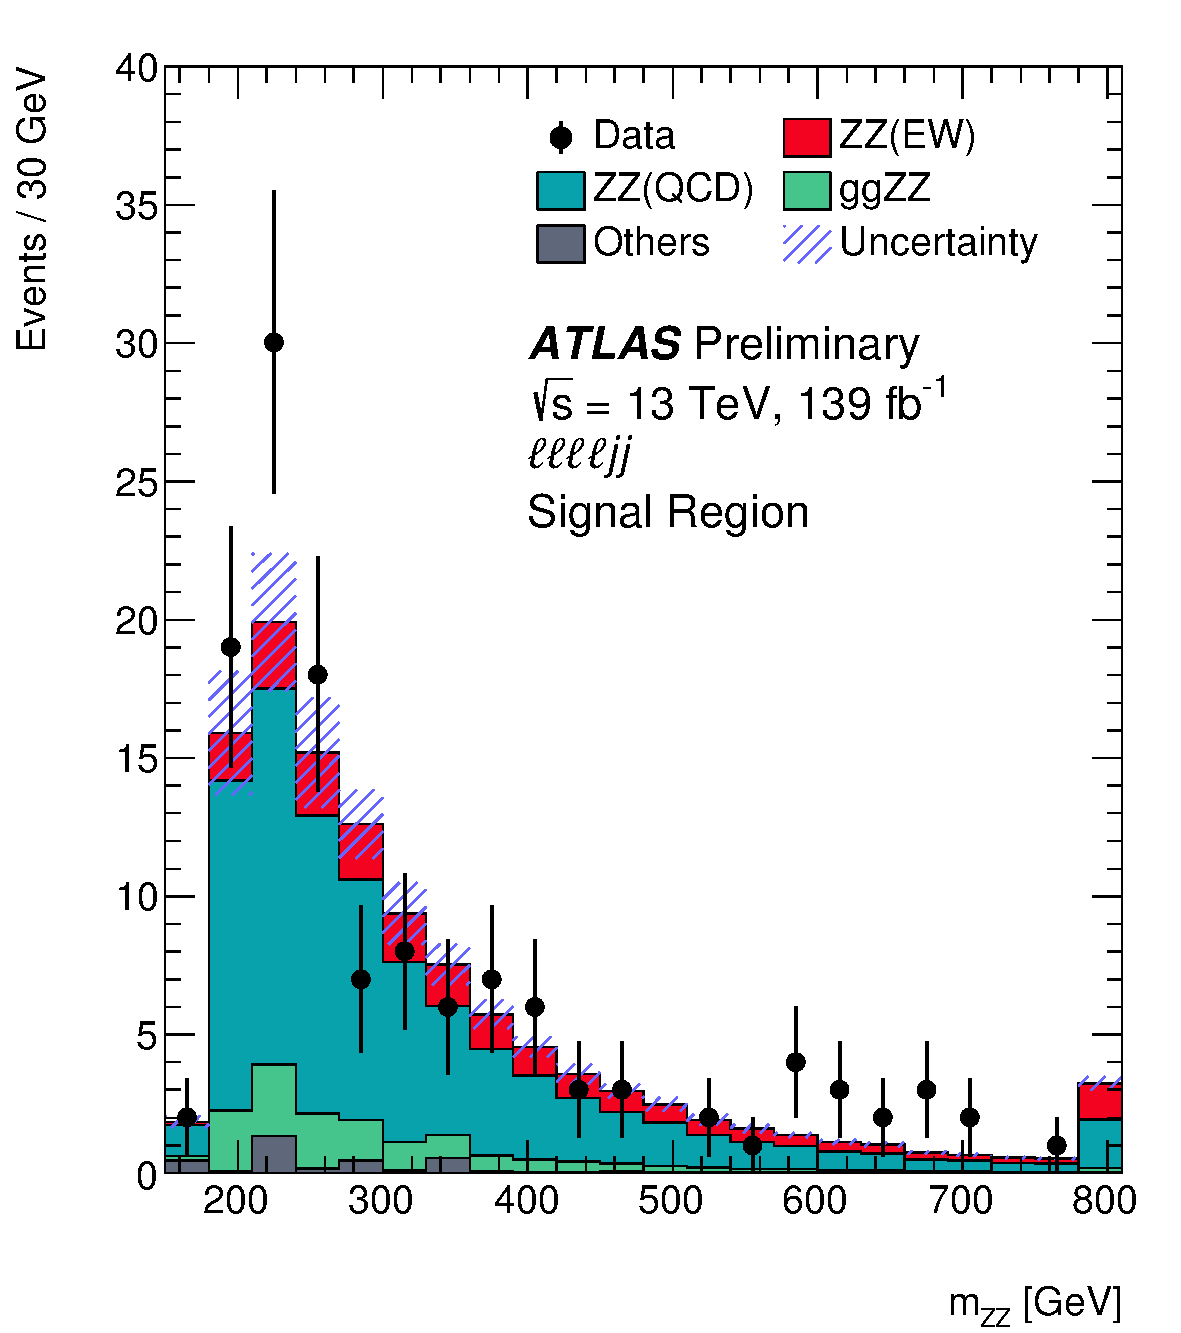
\includegraphics[width=0.4\textwidth]{figures/4l/MZZ_4l_SR_v1.pdf} \\
\end{center}
\caption{Observed and expected $m_{ZZ}$ distributions in the \lllljj channel SR. 
        The error bands include the expected experimental and theoretical uncertainties.
        The error bars on the data points show the statistical uncertainty on data.
        The contributions from the QCD and EW production of $ZZjj$ events are scaled by 0.96 and 1.35, respectively, 
        which correspond to the observed normalization factors in the statistical fit to the combined channel.
        The last bin includes the overflow events.
        }
\label{fig:mZZ}
\end{figure}

\begin{figure}[!htbp]
\begin{center}
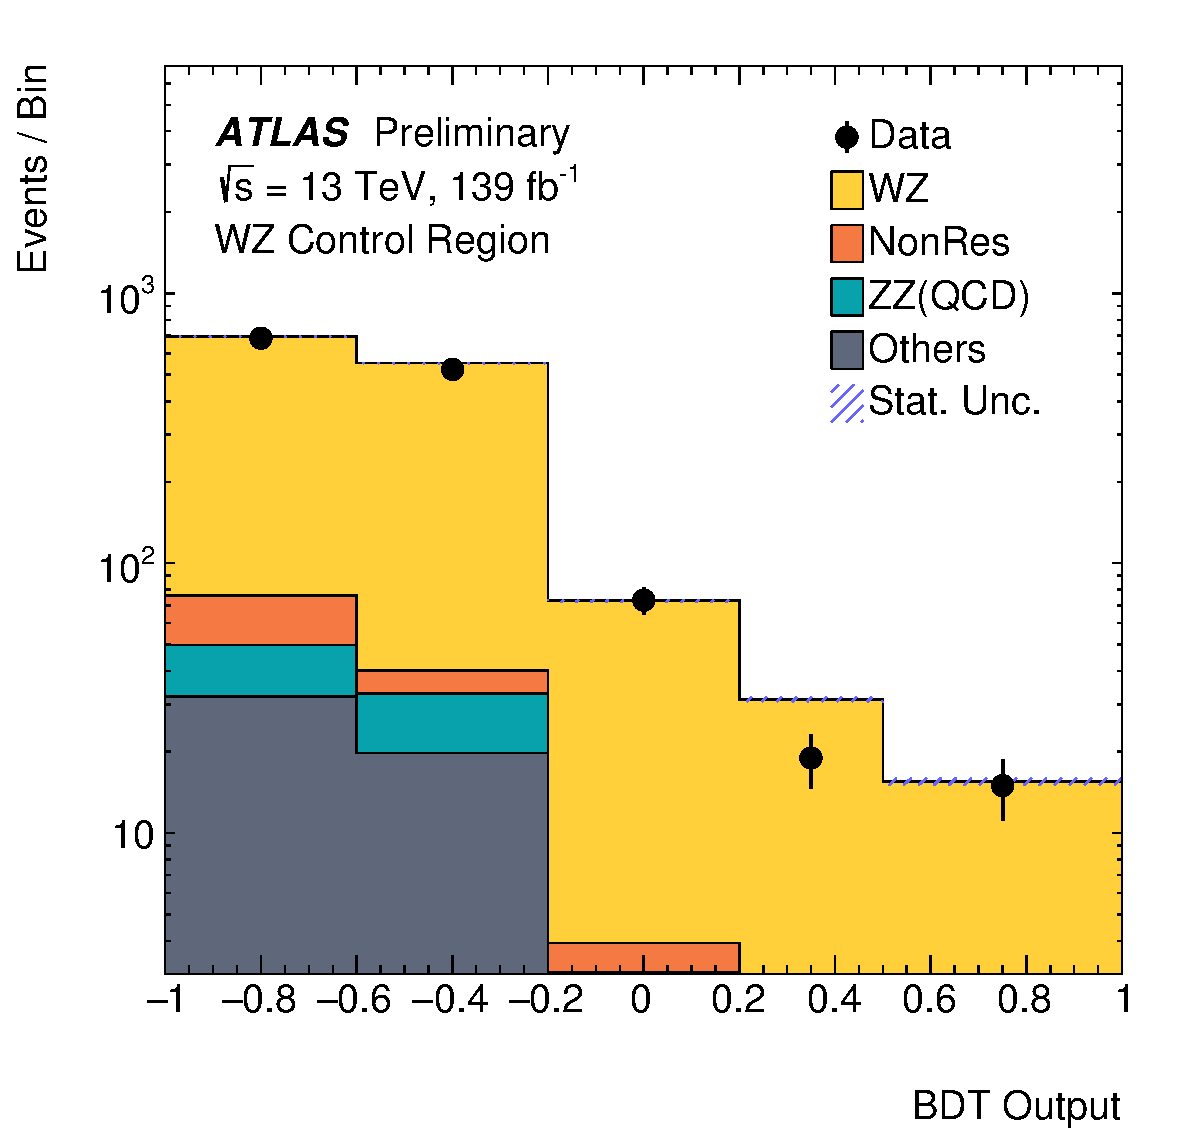
\includegraphics[width=0.4\textwidth]{figures/llvv/BDT_2l2v_3lCR.pdf} \\
%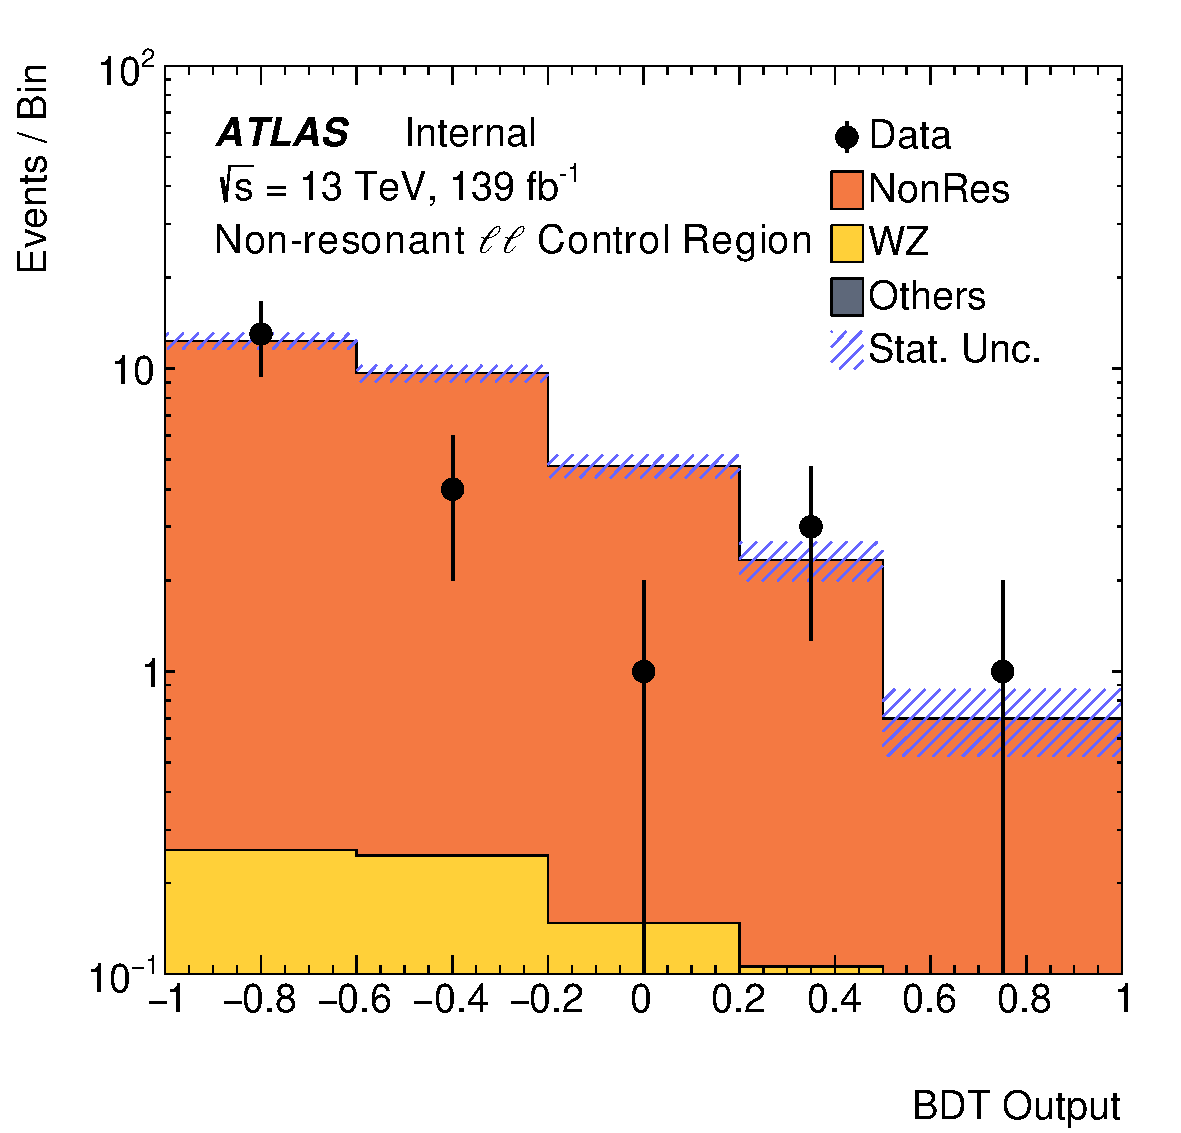
\includegraphics[width=0.325\textwidth]{llvv/BDT_2l2v_emCR.pdf} \\
\end{center}
\caption{Observed and expected multivariate discriminant distributions in the \llvvjj channel for 
        the $WZjj$
        %(left) and \nonresll (right)
        control region.
        The error bands only include the statistical uncertainties of the simulated samples.
        The error bars on the data points show the statistical uncertainty on data.
        }
\label{fig:MVA_2l2v_CR}
\end{figure}

\begin{figure}[!htbp]
\begin{center}
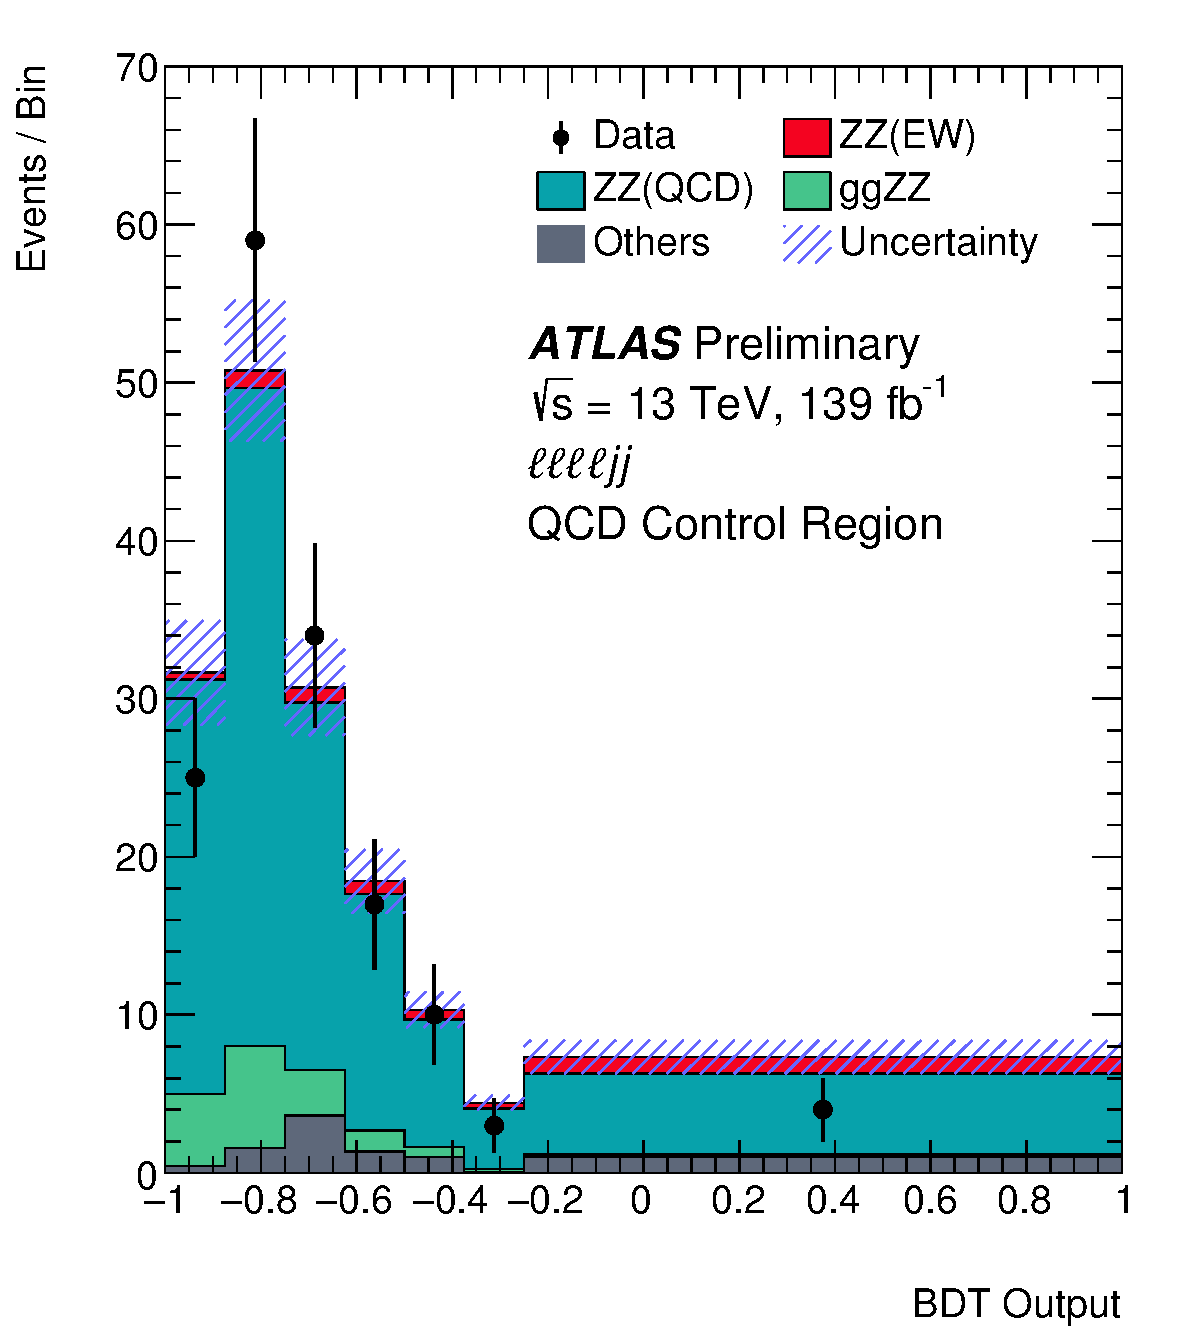
\includegraphics[width=0.325\textwidth]{figures/4l/BDT_4l_QCD_CR_postFit_v1.pdf}
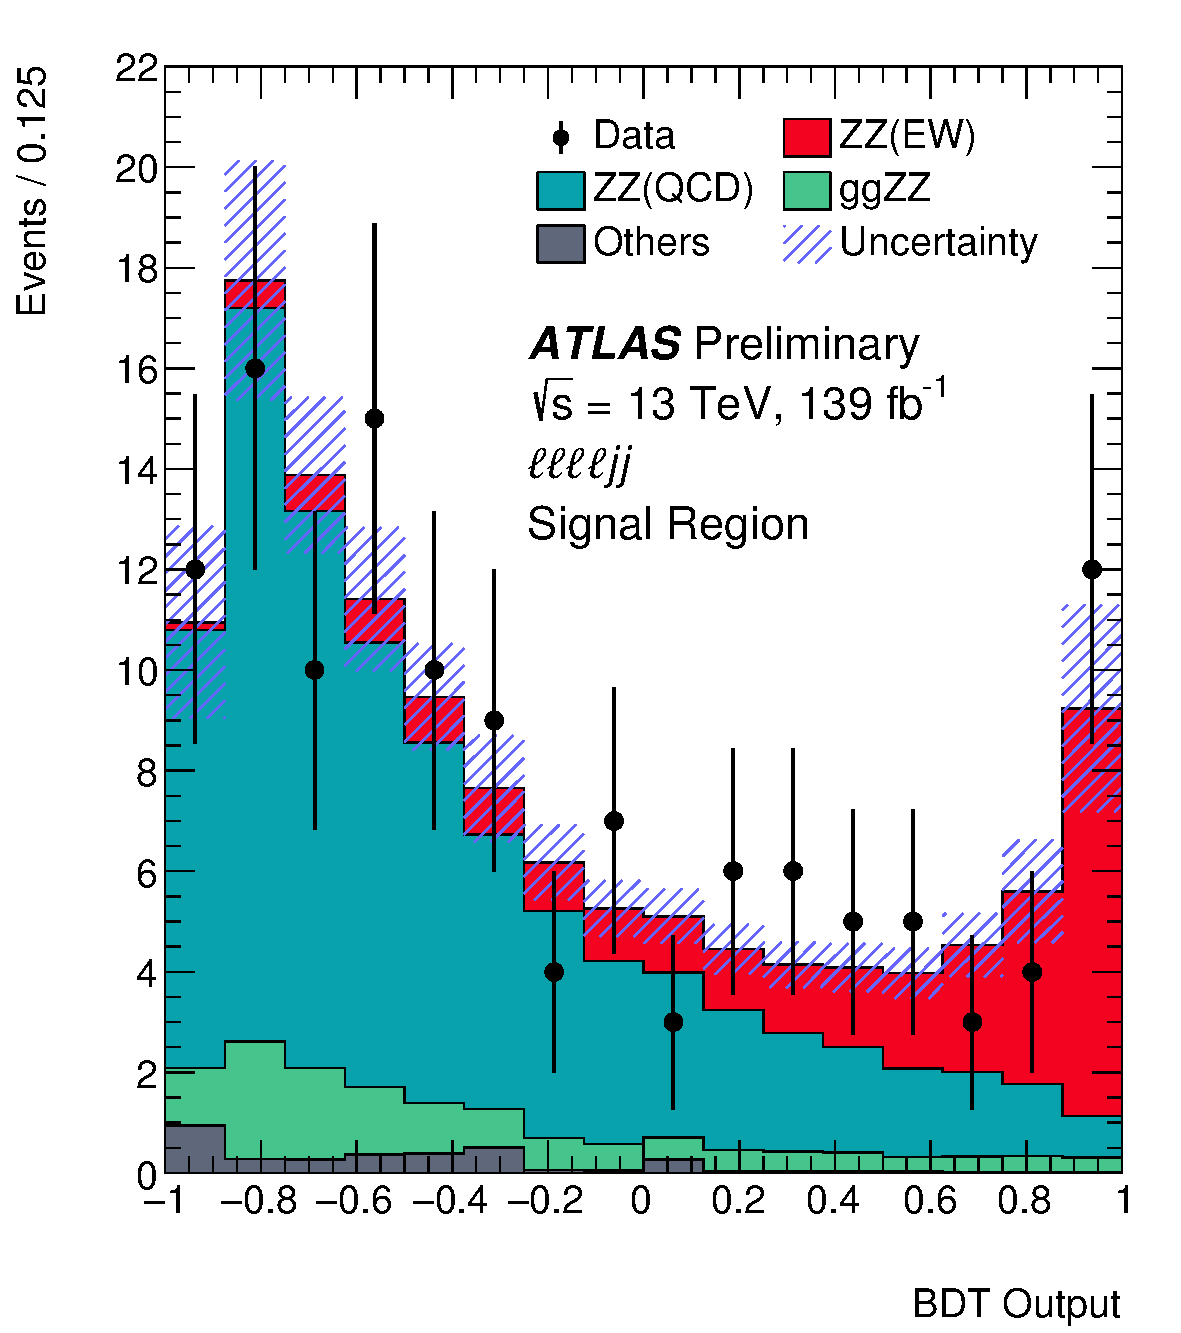
\includegraphics[width=0.325\textwidth]{figures/4l/BDT_4l_SR_postFit_v1.pdf}
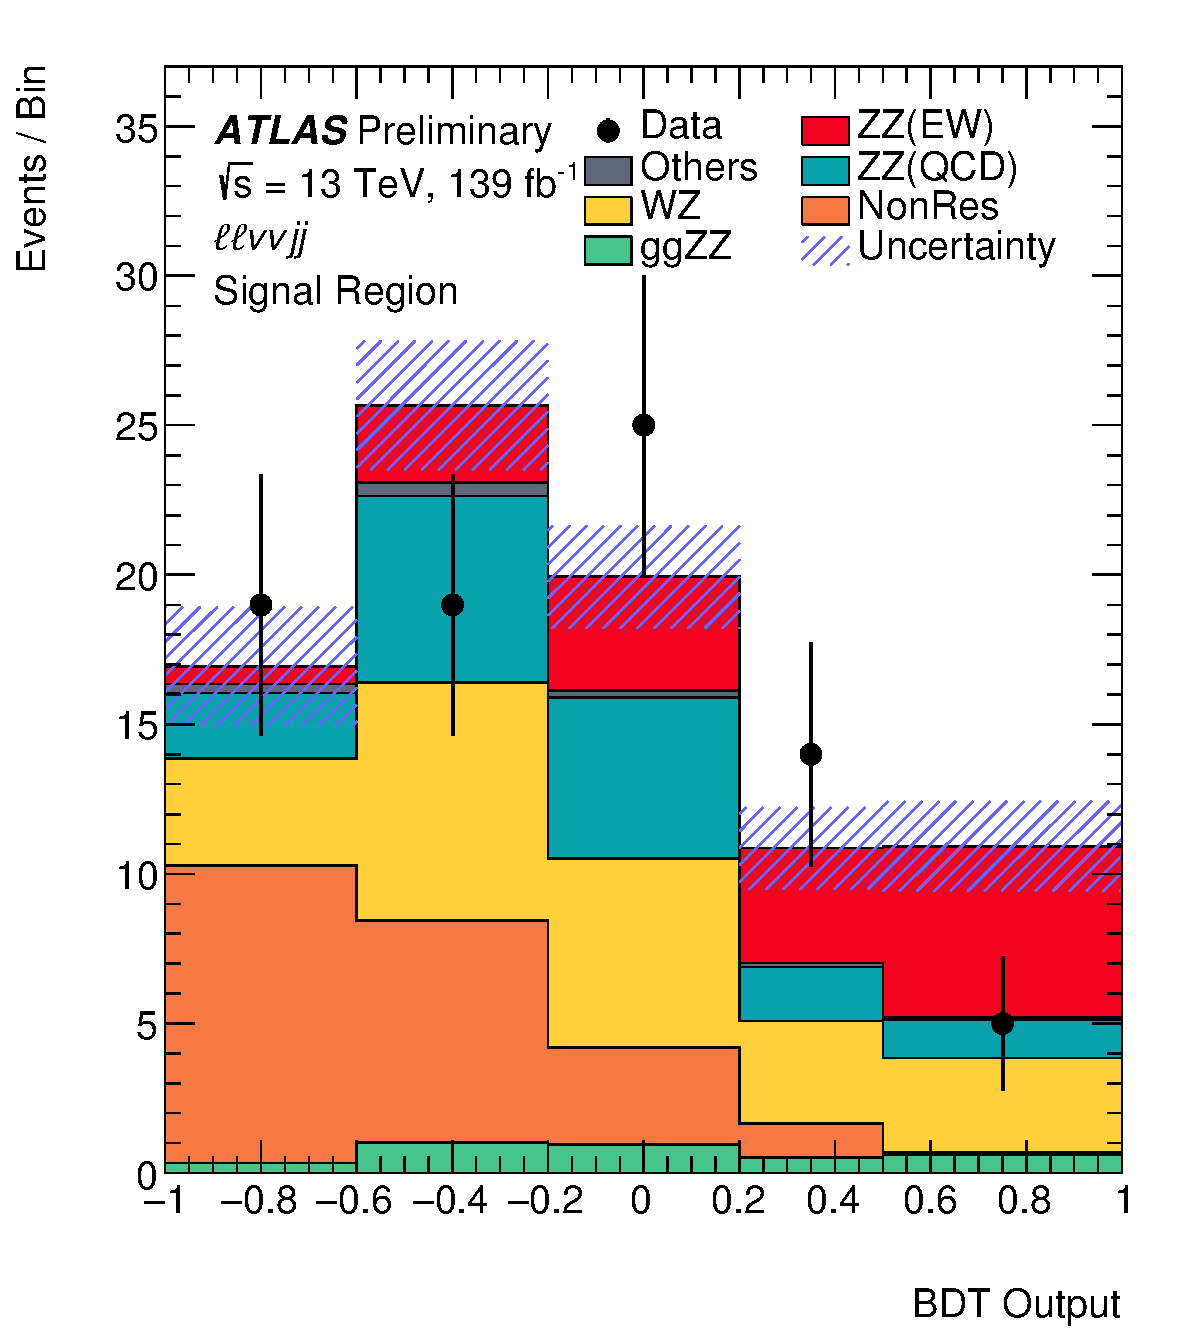
\includegraphics[width=0.325\textwidth]{figures/llvv/BDT_2l2v_SR_postFit_v1.pdf}\\
\end{center}
\caption{Observed and expected multivariate discriminant distributions after the statistical fit 
        in the \lllljj QCD CR (left), 
        and in the \lllljj (middle) and \llvvjj (right) signal regions.
        The error bands include the experimental and theoretical uncertainties, 
        as well as the uncertainties in \muEW and \muQCD.
        The error bars on the data points show the statistical uncertainty on data.
        }
\label{fig:MVA}
\end{figure}


%-------------------------------------------------------------------------------
\section{Conclusion}
\label{sec:conclusion}
This presentation summarizes the search for electroweak production of two jets in association with a $Z$-boson pair using the \llll and \llvv~decay final states of the two $Z$ bosons. The search uses 139 \ifb~of 13 \TeV~$pp$ collision data collected by the ATLAS detector at the LHC. In the optimised fiducial regions, the cross-sections for inclusive $ZZjj$ production are measured, with a total relative uncertainty of 11\% (28\%) for the \lllljj~(\llvvjj) channel, and found to be compatible with the SM predictions.
The search for electroweak production of two jets in association with a $Z$-boson pair is based on multivariate discriminants trained separately in each channel to enhance the separation between the signal and backgrounds. Combining both the \lllljj~and \llvvjj~channels, the background-only hypothesis is rejected with an observed (expected) significance of 5.5 (4.3) $\sigma$.
This gives the first observation of electroweak production of two jets in association with a $Z$-boson pair.
The measured cross-section for electroweak production in the fiducial region is $0.82\pm0.21$ fb,
corresponding to a signal strength of $1.35\pm0.34$, in agreement with the SM prediction.


%-------------------------------------------------------------------------------
\bibliography{bib/reference}
\bibliographystyle{ieeetr}

\end{document}
